\section{Aufbau}
\label{sec:Aufbau}

Der Versuch besteht aus einer Kupfer-Röntgenröhre, welche die in der Theorie beschriebene Röntgenstrahlung erzeugt, einem LiF-Kristall und einem Geiger-Müller-Zählrohr. Die erzeugte Röntgenstrahlung trifft auf den LiF-Kristall und wird an dessen Gitter-Struktur gestreut, sodass mit dem Geiger-Müller-Zählrohr die Intensität der Strahlung in Abhängigkeit vom Winkel aufgenommen werden kann.\\
Sowohl der Kristall, als auch das Zählrohr sind an einem Goniometer angebracht, sodass der Kristallwinkel und der Messwinkel individuell eingestellt werden können. Am Eingang des Geiger-Müller-Zählrohrs befindet sich eine waagerechte $\SI{1}{\milli\metre}$ Schlitzblende, an der bei der Absorptionsmessung die Absorber angebracht werden können.
Ein schematischer Aufbau des Röntgenspektrometers ist in Abbildung \ref{fig:Aufbau} dargestellt.

\begin{figure}
\centering
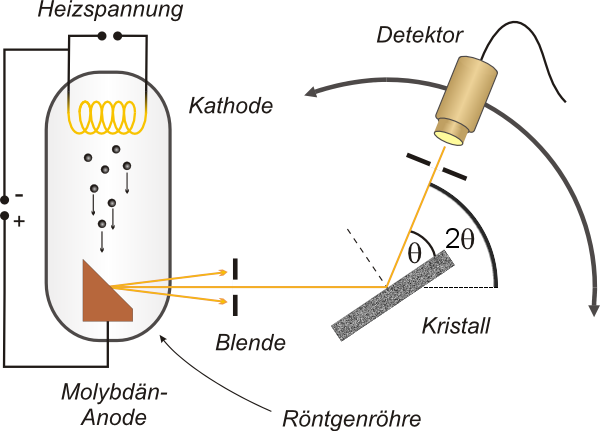
\includegraphics[scale = 0.5]{content/images/Aufbau.png}
\caption{Schematischer Versuchsaufbau des Röntgenspektrometers \cite{V602_Aufbau}.}
\label{fig:Aufbau}
\end{figure}
